% \iffalse meta-comment
%
% Copyright (C) 2017--2019 by Xiangdong Zeng <xdzeng96@gmail.com>
%
% This work may be distributed and/or modified under the
% conditions of the LaTeX Project Public License, either
% version 1.3c of this license or (at your option) any later
% version. The latest version of this license is in:
%
%   http://www.latex-project.org/lppl.txt
%
% and version 1.3 or later is part of all distributions of
% LaTeX version 2005/12/01 or later.
%
% This work has the LPPL maintenance status `maintained'.
%
% The Current Maintainer of this work is Xiangdong Zeng.
%
% \fi

%*********************************************************************
% fduthesis: 复旦大学论文模板
% 2019/04/03 v0.7d
%
% 重要提示:
%   1. 请确保使用 UTF-8 编码保存
%   2. 请使用 XeLaTeX 或 LuaLaTeX 编译
%   3. 请仔细阅读用户文档
%   4. 修改、使用、发布本文档请务必遵循 LaTeX Project Public License
%   5. 不需要的注释可以尽情删除
%   6. VS code编译有点问题用xetex->bibtex->xetex*2,否则参考文献会出错
%*********************************************************************

\documentclass[type=master,oneside]{fduthesis}
% 模板选项:
%   type = doctor|master|bachelor  论文类型,默认为本科论文
%   oneside|twoside                论文的单双面模式,默认为 twoside
%   draft = true|false             是否开启草稿模式,默认关闭
% 带选项的用法示例:
%   \documentclass[oneside]{fduthesis}
%   \documentclass[twoside, draft=true]{fduthesis}
%   \documentclass[type=bachelor, twoside, draft=true]{fduthesis}

\usepackage{cite}
\def\BibTeX{{\rm B\kern-.05em{\sc i\kern-.025em b}\kern-.08em
    T\kern-.1667em\lower.7ex\hbox{E}\kern-.125emX}}

% \usepackage{gbt7714}

\fdusetup{
  % 参数设置
  % 允许采用两种方式设置选项:
  %   1. style/... = ...
  %   2. style = { ... = ... }
  % 注意事项:
  %   1. 不要出现空行
  %   2. “=” 两侧的空格会被忽略
  %   3. “/” 两侧的空格不会被忽略
  %   4. 请使用英文逗号 “,” 分隔选项
  %
  % style 类用于设置论文格式
  style = {
    font = times,
    % 西文字体(包括数学字体)
    % 允许选项:
    %   font = garamond|libertinus|lm|palatino|times|times*|none
    %
    cjk-font = fandol,
    % 中文字体
    % 允许选项:
    %   cjk-font = adobe|fandol|founder|mac|sinotype|sourcehan|windows|none
    %
    % 注意:
    %   1. 中文字体设置高度依赖于系统。各系统建议方案:
    %        windows:cjk-font = windows
    %        mac:    cjk-font = mac
    %        linux:  cjk-font = fandol(默认值)
    %   2. 除 fandol 和 sourcehan 外,其余字体均为商用字体,请注意版权问题
    %   3. 但 fandol 字体缺字比较严重,而 sourcehan 没有配备楷体和仿宋体
    %   4. 这里中西文字体设置均注释掉了,即使用默认设置:
    %        font     = times
    %        cjk-font = fandol
    %   5. 使用 font = none / cjk-font = none 关闭默认字体设置,需手动进行配置
    %
    font-size = -4,
    % 字号
    % 允许选项:
    %   font-size = -4|5
    %
    fullwidth-stop = false,
    % 是否把全角实心句点 “.” 作为默认的句号形状
    % 允许选项:
    %   fullwidth-stop = catcode|mapping|false
    % 说明:
    %   catcode   显式的 “。” 会被替换为 “.”(e.g. 不包括用宏定义保存的 “。”)
    %   mapping   所有的 “。” 会被替换为 “.”(使用 LuaLaTeX 编译则无效)
    %   false     不进行替换
    %
    footnote-style = pifont*,
    % 脚注编号样式
    % 允许选项:
    %   footnote-style = plain|libertinus|libertinus*|libertinus-sans|
    %                    pifont|pifont*|pifont-sans|pifont-sans*|
    %                    xits|xits-sans|xits-sans*
    %
    hyperlink = none,
    % 超链接样式
    % 允许选项:
    %   hyperlink = border|color|none
    %
    % hyperlink-color = default,
    % 超链接颜色
    % 允许选项:
    %   hyperlink-color = default|classic|elegant|fantasy|material|
    %                     business|science|summer|autumn|graylevel|prl
    % 默认与西文字体保持一致
    %
    bib-backend = bibtex,
    % 参考文献支持方式
    % 允许选项:
    %   bib-backend = bibtex|biblatex
    %
    % bib-style = {gbt7714-plain.bst},
    bib-style = {numerical},
    % 参考文献样式
    % 允许选项:
    %   bib-style = author-year|numerical|<其他样式>
    % 说明:
    %   author-year  著者—出版年制
    %   numerical    顺序编码制
    %   <其他样式>   使用其他 .bst(bibtex)或 .bbx(biblatex)格式文件
    %
    % cite-style = {},
    % 引用样式
    % 默认为空,即与参考文献样式保持一致
    % 仅适用于 biblatex;如要填写,需保证相应的 .cbx 格式文件能被调用
    %
    bib-resource = {citelist.bib},
    % 参考文献数据源
    % 可以是单个文件,也可以是用英文逗号 “,” 隔开的一组文件
    % 如果使用 biblatex,则必须明确给出 .bib 后缀名
    %
    % logo = {fudan-name.pdf},
    % 封面中的校名图片
    % 模版已自带,通常不需要额外配置
    %
    % logo-size = {0.5\textwidth},      % 只设置宽度
    % logo-size = {{}, 3cm},            % 只设置高度
    % logo-size = {8cm, 3cm},           % 设置宽度和高度
    % 设置校名图片的大小
    % 通常不需要调整
    %
    % auto-make-cover = true
    % 是否自动生成论文封面(封一)、指导小组成员名单(封二)和声明页(封三)
    % 除非特殊需要(e.g. 不要封面),否则不建议设为 false
  },
  %
  % info 类用于录入论文信息
  info = {
    title = {论文标题},
    % 中文标题
    % 长标题建议使用 “\\” 命令手动换行(不是指在源文件里输入回车符,当然
    % 源文件里适当的换行可以有助于代码清晰):
    %   title = {最高人民法院、最高人民检察院关于适用\\
    %            犯罪嫌疑人、被告人逃匿、死亡案件违法所得\\
    %            没收程序若干问题的规定},
    %
    title* = {Thesis Title},
    % 英文标题
    %
    author = {xxx},
    % 作者姓名
    %
    % author* = {Your name},
    % 作者姓名(英文 / 拼音)
    % 目前不需要填写
    %
    supervisor = {xxx\quad 教授},
    % 导师
    % 姓名与职称之间可以用 \quad 打印一个空格
    %
    major = {软件工程},
    % 专业
    %
    degree = academic,
    % 学位类型
    % 允许选项:
    %   degree = academic|professional
    % 说明:
    %   academic      学术学位
    %   professional  专业学位
    %
    department = {软件学院},
    % 院系
    %
    student-id = {172120100**},
    % 作者学号
    %
    date = {YYYY 年 MM 月 DD 日},
    % 日期
    % 注释掉表示使用编译日期
    %
    % secret-level = ii,
    % 密级
    % 允许选项:
    %   secret-level = none|i|ii|iii
    % 说明:
    %   none  不显示密级与保密年限
    %   i     秘密
    %   ii    机密
    %   iii   绝密
    %
    % secret-year = {五年},
    % 保密年限
    % secret-level = none 时该选项无效
    %
    % 这里为了对齐强行加的空格, 有时间调下格式
    instructors = {
      {xxx \quad 教\quad 授},
      {x\quad x \quad 教\quad 授},
      {xxx \quad 副教授},
      {xxx \quad 副教授},
      {xxx \quad 副教授},
    },
    % 指导小组成员
    % 使用英文逗号 “,” 分隔
    % 如有需要,可以用 \quad 手工对齐
    %
    keywords = {不确定关系, 量子力学, 理论物理},
    % 中文关键字
    % 使用英文逗号 “,” 分隔
    %
    keywords* = {Uncertainty principle, quantum mechanics, theoretical physics},
    % 英文关键字
    % 使用英文逗号 “,” 分隔
    %
    clc = {TP311}
    % 中图分类号
  }
}

% 需要的宏包可以自行调用

% 需要的命令可以自行定义

\begin{document}

% 这个命令用来关闭版心底部强制对齐,可以减少不必要的 underfull \vbox 提示,但会影响排版效果
% \raggedbottom

% 前置部分包含目录、中英文摘要以及符号表等
\frontmatter

% 目录
\tableofcontents

% 插图目录
% \listoffigures
% 表格目录
% \listoftables

\begin{abstract}
  中文摘要
\end{abstract}

\begin{abstract*}
  english-abstract
\end{abstract*}

% 主体部分是论文的核心
\mainmatter

\chapter{绪论}
\section{研究背景}
测试参考文献~\cite{ASE10Rule}。
图片示例\ref{fig:fig1}

\begin{figure}[htb]
    \centering
    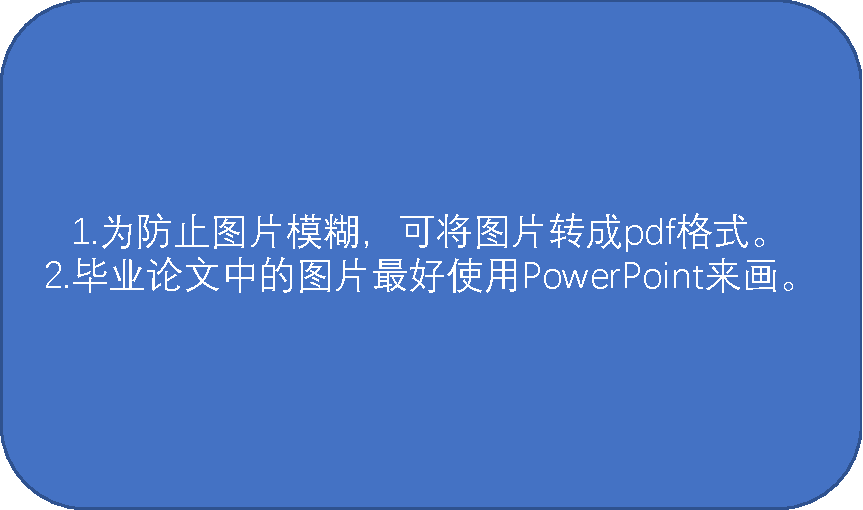
\includegraphics[width=\textwidth]{image/fig1.pdf}
    \caption{代码示例的抽象语法树} 
    \label{fig:fig1} 
\end{figure}

\chapter{背景知识和相关技术}
\section{研究背景}
测试参考文献~\cite{ASE10Rule}。
图片示例\ref{fig:fig1}

\begin{figure}[htb]
    \centering
    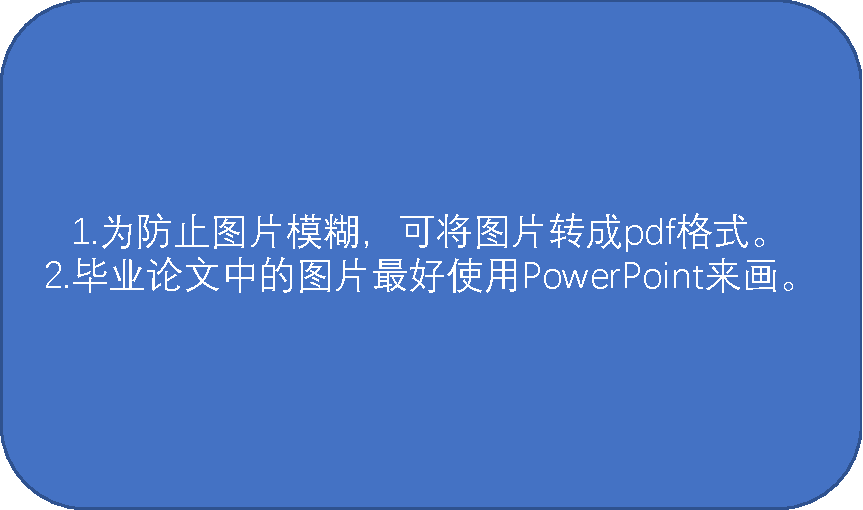
\includegraphics[width=\textwidth]{image/fig1.pdf}
    \caption{代码示例的抽象语法树} 
    \label{fig:fig1} 
\end{figure}

\chapter{实现方法}
\section{研究背景}
测试参考文献~\cite{ASE10Rule}。
图片示例\ref{fig:fig1}

\begin{figure}[htb]
	\centering
	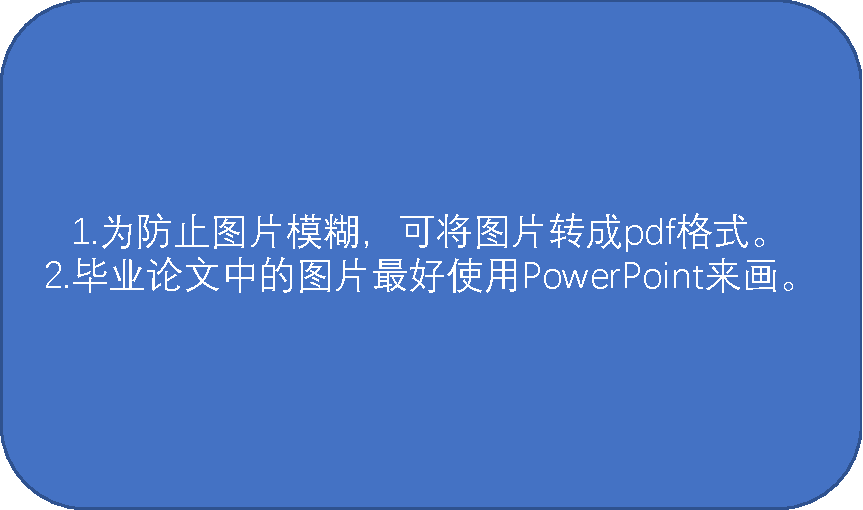
\includegraphics[width=\textwidth]{image/fig1.pdf}
	\caption{代码示例的抽象语法树} 
	\label{fig:fig1} 
\end{figure}

\chapter{实验}
\section{研究背景}
测试参考文献~\cite{ASE10Rule}。
图片示例\ref{fig:fig1}

\begin{figure}[htb]
    \centering
    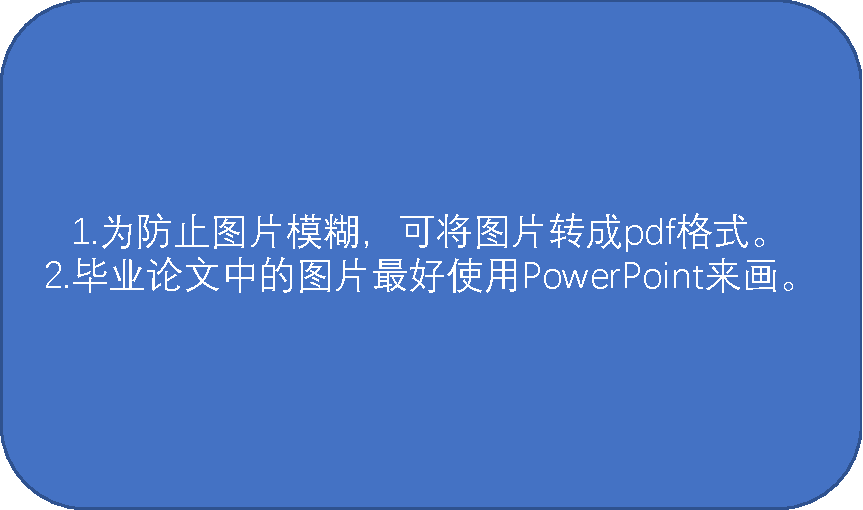
\includegraphics[width=\textwidth]{image/fig1.pdf}
    \caption{代码示例的抽象语法树} 
    \label{fig:fig1} 
\end{figure}

\chapter{讨论}
\section{研究背景}
测试参考文献~\cite{ASE10Rule}。
图片示例\ref{fig:fig1}

\begin{figure}[htb]
    \centering
    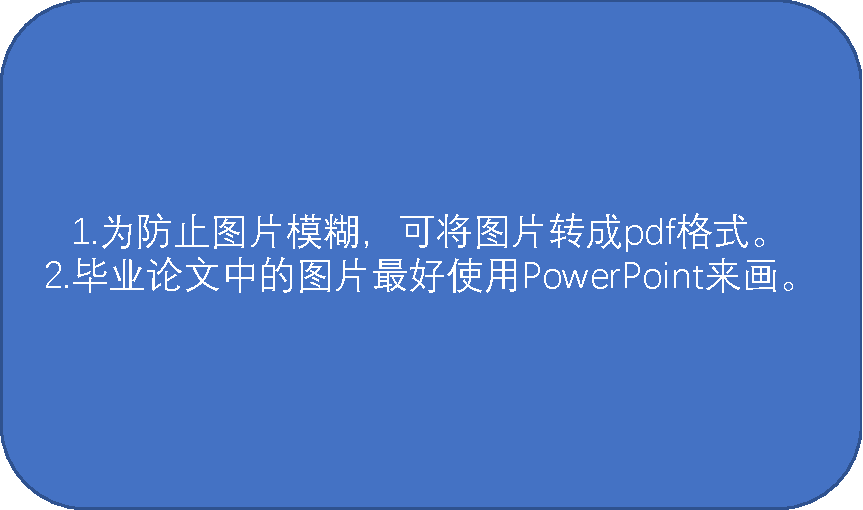
\includegraphics[width=\textwidth]{image/fig1.pdf}
    \caption{代码示例的抽象语法树} 
    \label{fig:fig1} 
\end{figure}

\chapter{结论}
\section{研究背景}
测试参考文献~\cite{ASE10Rule}。
图片示例\ref{fig:fig1}

\begin{figure}[htb]
    \centering
    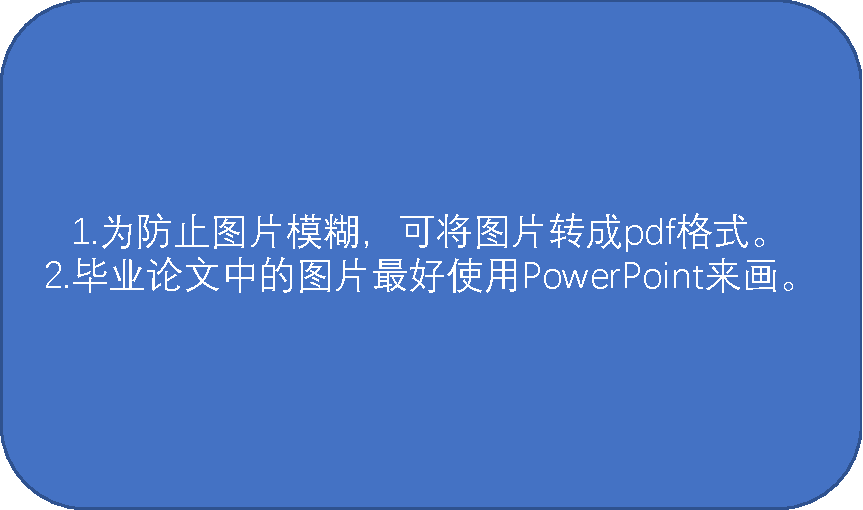
\includegraphics[width=\textwidth]{image/fig1.pdf}
    \caption{代码示例的抽象语法树} 
    \label{fig:fig1} 
\end{figure}

% 后置部分包含参考文献、声明页(自动生成)等
\backmatter

\renewcommand\refname{参考文献}

\bibliography{citelist}

\chapter{致谢}
% \addcontentsline{toc}{chapter}{致谢}
谢谢

% 专硕同学可以注释
\chapter*{攻读硕士学位期间发表论文情况}
\begin{enumerate}
    \renewcommand{\labelenumi}{[\theenumi]}
    \item xxxx. 已录用. 2019.
\end{enumerate}


\end{document}
